\section{Introduction}
The goal of physics is to create a mathematical model that accuratly describes a phyuical system.
Different types of theories may be appropriate for describing different energy and length scales.
Interactions between realitivly large and slow objects, all of those we encounter in day-to-day life, fall under the purvue of Classical Mechanics.
When these large objects are accelerated to speeds approaching the speed of light, Relativistic Mechanics describes their interactions well.
When one instead views the world at the smallest scales, one finds that the universe is made up of a few types of fundemental particles which are identical and indistingishable.
The behavior of this fundemental matter at low energies is given by Quantum Mechanics, while at high energies it is described by Quantum Field Theory.
Quantum Field Theory (QFT) represents the combination of relativity and quantum mechanics.

\TCR{add bridge to standard model}

\subsection{The Standard Model}
The Standard Model of particle physics represents the most complete description of fundemental interactions to date, surviving over 70+ years of theoratical and experimental scrutiny.
The Standard Model, shown in Figure~\ref{fig:standard_model_particles}, combines Quantum Field Theories of the ElectroWeak forces (Electrodynamics) and the Strong interaction (Chromodynamics) into a unified framework.
Each interaction has its own force carrier, with the strong, electromagnetic, and weak forces being mediated by the gluon, photon, and W$^{\pm}$+Z bosons respectivly.


\begin{figure}
    \centering
    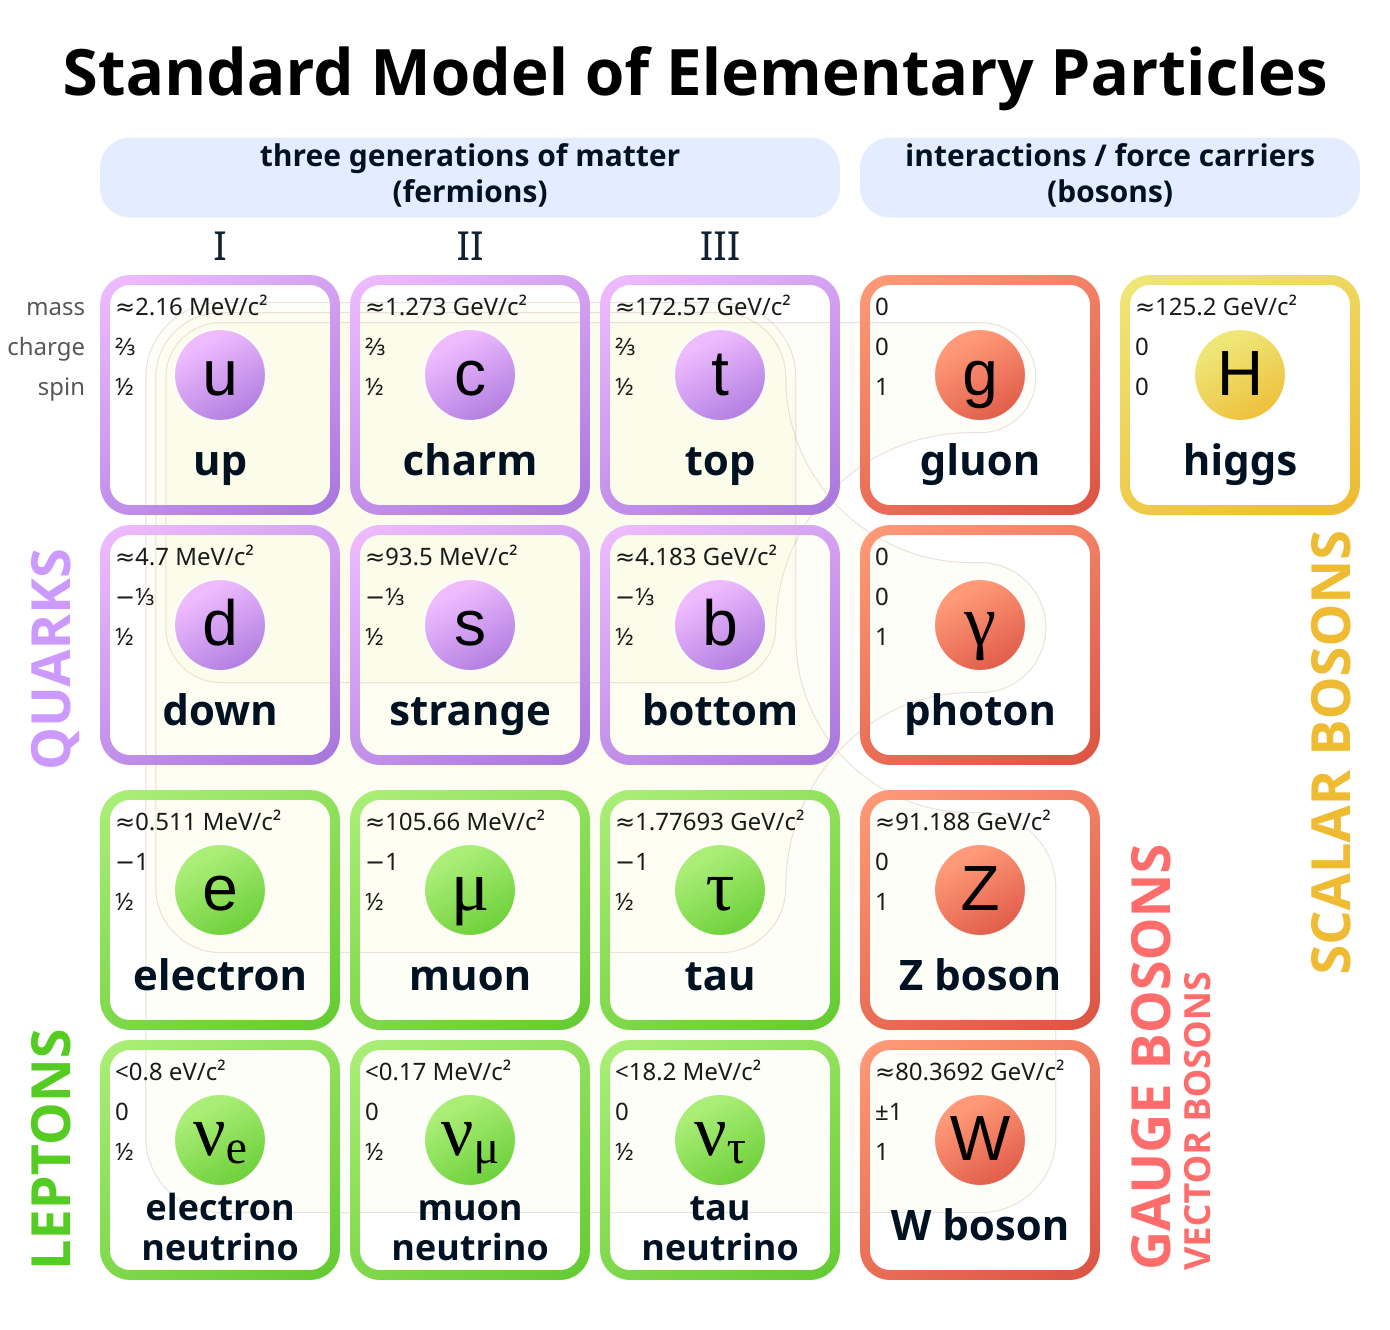
\includegraphics[
        width=0.85\textwidth,
        alt={Diagram of the Standard Model showing three generations of quarks
        and leptons, along with gauge bosons and the Higgs boson.}
    ]{chapters/introduction/figures/the_standard_model/standard_model_of_elementary_particles.pdf}
    \caption{The elementary particles and force carriers of the Standard Model.
    Adapted from Ref.~\cite{WikimediaCommonsStandardModel}.}
    \label{fig:standard_model_particles}
\end{figure}

\input{chapters/introduction/sections/qcd.tex}
\subsubsection{Jets}

Placeholder text for this section.

\subsubsection{Parton Distribution Functions}

Placeholder text for this section.

